\documentclass[11pt,Chicago]{uuthesis}
\usepackage{amssymb}
\usepackage{thesis}
\usepackage{graphicx}
\usepackage{amsmath}

\usepackage{hyperref}
\hypersetup{
  % bookmarks=true,         % show bookmarks bar?
    unicode=false,          % non-Latin characters in Acrobat’s bookmarks
    pdftoolbar=true,        % show Acrobat’s toolbar?
    pdfmenubar=true,        % show Acrobat’s menu?
    pdffitwindow=false,     % window fit to page when opened
    pdfstartview={FitH},    % fits the width of the page to the window
    pdftitle={Resting State Functional MRI Analysis by Graphical Model},
    pdfauthor={Wei Liu},     % author
    pdfsubject={Ph.D. Dissertation},   % subject of the document
    pdfcreator={Wei Liu},   % creator of the document
    pdfproducer={Producer}, % producer of the document
    pdfkeywords={Ph.D. thesis, functional MRI, connectivity}, % list of keywords
    pdfnewwindow=true,      % links in new window
    colorlinks= true,       % false: boxed links; true: colored links
    linkcolor=blue,          % color of internal links
    citecolor=blue,        % color of links to bibliography
    filecolor=magenta,      % color of file links
    urlcolor=cyan           % color of external links
}


% The packages 'flafter' and 'afterpage' will aid figure placement
\usepackage{flafter}
\usepackage{afterpage}

\usepackage{color}
\definecolor{darkgreen}{rgb}{0.0, 0.4, 0.0}
\definecolor{darkblue}{rgb}{0.0, 0.0, 0.6}
\definecolor{darkred}{rgb}{0.6, 0.0, 0.0}

% Make sure subfigures have parentheses around them everywhere
%\renewcommand\thesubfigure{(\alph{subfigure})}
% Make sure subfigures have parentheses around them everywhere
%\renewcommand\thesubfigure{(\alph{subfigure})}

\usepackage{lscape}
%\usepackage{diagram}
%\usepackage{tgrind}
\let \tenrm = \rm 		% This is used in fig*.tex
%\includeonly{}                    % Only front matter and back matter
%\includeonly{chap1}               %  plus chapter 1
%\includeonly{chap2}                %  plus chapter 2
%\includeonly{chap3}                %  plus chapter 3
%\includeonly{appA}                %  plus chapter 3
%\includeonly{chap1,chap2,chap3,chap4}   %  plus all chapters
%\includeonly{chap1,chap2,chap3,chap4,appA}   %  plus all chapters & appendix
%
%\tracingstats=2                % show TeX memory usage
\title{TITLE LINE 1\protect\\ TITLE LINE 2}
\author{First M. Last}
\thesistype{thesis} % or dissertation
\graduatedean{Charles A. Wight}
\department{Department Name}
\degree{Master of Science}  % of Doctor of Philosophy
\departmentchair{First M. Last}
\committeechair{First M. Last}
\firstreader{First M. Last}
\secondreader{First M. Last}
%\thirdreader{First M. Last}
%\fourthreader{First M. Last}
\chairtitle{Professor}
\submitdate{Month Year}
\copyrightyear{Year}
% Chapter is one level, section and subsection are the next two levels.
\fourlevels
%\dedication{For my horse, Dixie, etc. A few lines only.}
 \inputpicturetrue  % By Jeff McGough. See uuguide and private thesis.sty
%\inputpicturefalse % To NOT produce pictures, uncomment this line
\begin{document}
%% Comment out items by inserting a percent % character
\frontmatterformat
\titlepage
\copyrightpage
\committeeapproval
%\readingapproval
\preface{abstract}{Abstract}
%\dedicationpage
%\begin{epigraph}
%``Nature is trying very hard to make us succeed, but nature does not depend on us. We are not the only experiment.''
%\begin{flushright} -- R. Buckminster Fuller \par\end{flushright}
%\end{epigraph}
\setcounter{tocdepth}{4}    %How many levels to include in TOC
\addtocontents{toc}{\protect\sloppy}    %Keeps long chapters within page # margins
\tableofcontents
\listoffigures
\listoftables
%
% Optional front page, made from source "notation.tex".
% If you don't need it, then don't use it.
%
%\optionalfront{Notation and Symbols}{\input{notation.tex}}
\preface{acknowledge}{Acknowledgments}
\maintext       % Start normal page numbering. Parts and chapters follow.
\chapter{Chapter 1 Title}\label{chap1}
%\fixchapterheading % Use this if section follows chapter immediately

Text

\section{Section Title}  % level 2
Text 
   \begin{table}[b]
    \caption{Experimental values for toe parameters while perching.}
    \label{tab:footData}
    \begin{center}
    \begin{tabular}{c|c|c|}
      \cline{2-3}
      % after \\: \hline or \cline{col1-col2} \cline{col3-col4} ...
      {} & \textbf{33\,mm Perch} & \textbf{49\,mm Perch} \\\hline
      \multicolumn{1}{|c|}{\textbf{$\delta$}} & 37\,mm & 31\,mm \\
      \multicolumn{1}{|c|}{\textbf{$\theta_1$}} & $(62^\circ+52^\circ)/2=57^\circ$ & $(56^\circ+39^\circ)/2=47^\circ$ \\
      \multicolumn{1}{|c|}{\textbf{$\theta_2$}} & $(60^\circ+66^\circ)/2=63^\circ$ & $(51^\circ+53^\circ)/2=52^\circ$ \\
      \multicolumn{1}{|c|}{\textbf{$\theta_3$}} & $(66^\circ+71^\circ)/2=68^\circ$ & $(57^\circ+61^\circ)/2=59^\circ$ \\
      \hline
    \end{tabular}
    \end{center}
   \end{table}
Text 
   \begin{figure}[t]
      \centering
      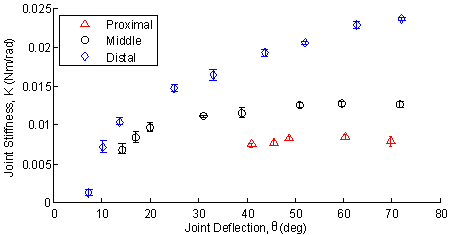
\includegraphics[width=.7\textwidth]{chap1img/jointDeflection4.pdf}
      \caption[Joint stiffness as a function of deflection]{Joint stiffness as a function of deflection. Values are calculated using the mean joint deflections reported in Table \ref{tab:deflect}. Error bars show the range of K values possible with all permutations of $\pm\sigma$ in joint deflection. Stiffness is nonlinearly related to deflection and increases as the toe deflects further.}
      \label{fig:jointDeflect}
   \end{figure}

\subsection{Subsection Title} %level 3
Text  
\chapter{Background and related works}
\label{chap:bg}
% This chapter will cover: Effect of preprocessing. SPM smoothing, Random field
% theory for enforcing smoothing.

% a very high level overview.
The human brain is organized into distributed functional modules that work
independently but also interact with one another during cognitive
activity. There appears two principles of how the brain function is organized:
functional integration and functional
specialization~\cite{friston2007statistical}. Functional specialization assumes
the modules that process a particular cognitive activity can be localized to an
anatomical region in the brain. In functional specialization, one studies the
relationship of specific anatomical regions and cognitive activity. However, the
brain regions or functional modules do not work alone. They interact with each
other in a complex and dynamic way. Functional integration focuses on such
interactions.

% what will be covered in this chapter.
This chapter provides background information about the current research
exploring brain's functional network using rs-fMRI. I will begin with the
relationship between brain activity and fMRI, and give the definitions of
functional connectivity and functional network. Then I will survey various
classes of methods for estimating functional connectivity and networks.

%% Brain network organization, anatomical/functional connectivity, fmri BOLD,
%% oxygen, task, resting-state, functional network
\section{Resting-state functional networks}
% the interaction: anatomical connectivity and functional connectivity. 
The interactions among various functional modules of the brain can be
represented by the connectivity among anatomical regions. Two sets of MRI
techniques are widely used for mapping the \emph{in vivo} connectivity of the
human brain. Diffusion MRI, or more specifically, diffusion tensor imaging
(DTI), as a structural imaging technique, detects the anisotropy of the neural
axons in the brain's white matter by measuring the diffusion of water
molecules. Such anisotropy is used for identifying the anatomical connectivities
between two regions in the brain's white
matter~\cite{jirsa2007handbook}. Functional MRI (fMRI) imaging, in contrast,
serves to explore the functional links between two regions of interest in
brain's gray matter. The functional connections are the actual flow of
information through the anatomical links represented by the DTI. Researchers
have demonstrated the correlation between the anatomical and functional
connections. Such correlation is an indication that functional connectivity is
physically constrained and modulated by the structural
connectivity~\cite{honey2009predicting}. However, functional and structural
connectivity are not exactly equal, suggesting the dynamic characteristics of
the functional patterns depend on the brain's state. The work in this dissertation
is focused on functional connectivity.

% fmri intro, BOLD, oxygen, task-based. 
Information is transferred in axons between neurons by the release of
neurotransmitter molecules at synapses. The interactions between
neurotransmitter and receptors consume energy. Because energy is produced by
oxidative metabolism, increased synaptic activity will also increase local
demand for delivery of oxygen. This, counter intuitively, increase the local
blood flow, and increases the $T_2^*$ image
intensity~\cite{lewin2003functional,stroman2011essentials}. Even deoxygenated
hemoglobin decreases during neural activity, MR signal increases. This is
because more oxygen is supplied to the brain region than is consumed.

Haemoglobin have different magnetic property when it is bound to oxygen. This
changes the local distortions of a magnetic field, which can be detected by MRI
scanner. The relaxation times depends on the level of blood oxygenation, and the
MRI signal depends on the relaxation time, and is called blood oxygenation
level-dependent (BOLD) signal.

To understand the response of BOLD signal to a general stimulus signal, we need
to know its response to a very short impulse signal, namely, a $\delta$
function. It is noted that the BOLD signal have about two seconds lags after the
onset of stimulus. This initial dip is attributed to the transient increase of
deoxygenated hemoglobin. After 4 to 6 seconds, the demand due to increase neuro
activity results in an increased inflow of oxygenated blood, and it reaches the
highest point. After the neuro activity stops, the BOLD goes below the baseline
level. It takes about twenty seconds for the BOLD to go back to the baseline in this
\emph{poststimulus undershot}. The balloon model \cite{buxton1998dynamics} is
used to explain this extended period. The response function to a $\delta$
function is called the Hemodynamic response function (HRF). The response of a
general boxcar function, would be the convolution of the boxcar function and the
HRF.

Because the resolution of fMRI is much higher than the single cell or neuron,
the BOLD signal reflects the energy demands of neuropopulation that fire
together with a common functional purpose~\cite{huettel2004functional,
  jezzard2003functional}. Besides fMRI, other techniques are also used for
mapping the functions of the brain. They differ in terms of both their temporal
and spatial resolution. In general, electrophysiological methods, such as
electroencephalography (EEG) or the associated magnetic version
magnetoencephalography (MEG), record the neural events in real time; hence,
these methods have relatively high temporal resolution. On the other hand, fMRI
and positron emission tomography (PET) detect the change of blood flow due to
neuronal information processing, and have high spatial resolution (1-5 mm), but
lower temporal resolution because of the delayed haemodynamic changes.

% functional connectivity and functional network.
fMRI was initially discovered as a tool to map the brain's activity for subjects
in specific cognitive experiments. One compares the BOLD signal at a specific
region in the brain with the paradigm task signal. Because of the nature of the
haemodynamics of the blood, the paradigm task signal is the convolution of the
original paradigm function (for example, a boxcar function) with the
haemodynamic response function (HRF). Later, researchers found that the BOLD
signals can be used not only to detect the functional patterns in
stimulus-guided experiments, but also to explore the co-activation of the brain
when the subjects are not performing cognitive
tasks~\cite{biswal1995functional}. In such experiments, the primary goal is to
identify the functional connectivity between pairs of regions in the
brain. Functional connectivity is defined as the temporal dependence of neuronal
activity patterns of spatially remote (or anatomically separated) brain
regions~\cite{friston1994functional, worsley_analysis_1995,
  friston1994analysis}. The temporal dependence is typically measured by the
linear correlation across all time points. Although the temporal correlation
within the BOLD signal of a single region or voxel violates the independence
assumption of the time point samples, this temporal correlation is often safely
ignored. Alternatively, one can also identify functional connectivity by
transforming the signals into the frequency domain and using the coherence of
two signals at a certain frequency band. The coherence as similarity measurement
is equivalent to band pass filtering the original BOLD signal and computing the
linear correlation~\cite{cordes2000mapping, cordes2001frequencies}.

% Define a functional network. 
The pairwise correlation or coherence only measure the functional connectivity
between regions as a local measurement. As the whole brain is organized as a
complex system with many such pairwise interactions, it is of interest to find
out those regions with similar patterns of neuronal activity. A functional
network, or functional system (hereafter used interchangeably), is a collection
of separate anatomical regions that have similar patterns of activity measured
by BOLD signal. The regions within a functional system may have direct or
indirect information flow among them. Together the system serves one or more
cognitive tasks. An anatomical region may participate in different functional
systems during different cognitive tasks.

%% [ Various levels. Task, resting, Cognitive disease. Mental disorder. Low
%% frequency. Correlation.
The correlated fluctuation of multiple brain regions not only occurs in
stimulus-evoked experiments, but also in experiments where the participants rest
passively without any cognitive activity. Therefore, the resting-state fMRI
(rs-fMRI) becomes a powerful tool for probing such intrinsic activity in a
resting brain~\cite{raichle2001, fox2007spontaneous}. The original name of the
rs-fMRI is not accurate, since the brain is not truly in a resting state even
without any cognitive activity. The resting brain consumes about 20 percent of
the energy of the whole body, but it occupies about only 5 percent of the body
mass~\cite{fox2005human}. The study of the functional organization of the
resting brain provides new insights into how functional connectivity relates to
cognitive psychology and neurodegenerative diseases.  Because the pathologic
conditions appear to be reflected by the interactions within or between the
functional systems, the rs-fMRI study also holds valuable diagnostic and
prognostic information towards various neurological or psychiatric diseases
including Alzheimer's diseases, depression, and
schizophrenia~\cite{fox2007spontaneous, greicius2007resting,
  greicius2003functional}, etc. The reason for this spontaneous activity is
largely unknown, although some researchers reasonably postulate that it is a
predictive intrinsic response to the unknown events in the outside
environment~\cite{deco2010emerging}.

% preprocessing. motion correction. global signal regression? slice timing
% correction, nuisance parameter regression (GM, WM, CSF), registration.
\section{Preprocessing fMRI data}
Due to the noise and artifacts in fMRI data, multiple preprocessing steps are
typically taken before the real analysis starts. The preprocessing steps include
motion correction, slice timing correction, spatial and temporal filtering,
registration between structural images and functional images, registration
to the standard template, and removing physiological noise, etc.

Because of a subject's head movements during the scan, the volumes at various
time points are usually not perfectly aligned. A rigid body registration is
usually done between the volumes at different time points, with either the first
volume or the middle volume as a reference. This is called motion
correction. After correction, the same voxel coordinate is assumed to map to the
same brain structure across all time points, although the correction is often
not perfect. The motion correction parameters of each volume are often used as
independent variables for a regression in order to remove the motion effect. The
first few time points are usually discarded in case the scanner is not in a
stationary state.

Slice timing correction is needed because each slice of fMRI volume is not
scanned at the same time. Figure \ref{fig:slicetiming} shows the shifted time of
scans for different slices and the method of interpolation.  The shifted time
will give suboptimal experiment results during the analysis, especially for the
event-based experiments. One typically uses an interpolation step to obtain a
volume in which all slices are at the same time point. Care must be taken for
the ordering of the slices as the ordering is scanner dependent.


Because of the physiological process of the BOLD signal, most of the interesting
information is concentrated at the low frequency range of the signal (0.01 --
0.1 Hz). The temporal band-pass filter is usually applied to remove the very low
frequency (below 0.01 Hz) and higher frequency (above 0.1 Hz). Also, due to the
spatial process of fMRI data acquisition, neighboring voxels typically have
similar signal patterns. The statistical parametric mapping
method~\cite{friston2007statistical} makes use of this spatial dependency by
applying a spatial Gaussian filter, and further enforces the smoothness of the
signal on the spatial domain. This filtering increases the SNR, but inevitably
discards finer patterns with size smaller than the smoothing kernel. Chapter
\ref{chap:method1} and Chapter \ref{chap:method2} will discuss more principal
methods that model this spatial dependency with no spatial smoothing, or very
small, conservative smoothing.

In order to report the experiment results in a standard way such that others can
understand, the structural images and functional images are both registered to a
standard template, such as the MNI 152
template~\footnote{http://www.bic.mni.mcgill.ca/ServicesAtlases/ICBM152NLin2009}. The
functional images are first registered to structural images of the same subject
by a rigid body transformation. The structural images are then transformed to
the standard template by affine transformation. Because of the plasticity of the
brain anatomy, the registration of the subject's structural image may need
nonlinear transformation to register to the
template~\cite{jenkinson2012fsl}. After the structural images are registered to
the template, the functional images will also be brought to the template space
by the same transformation. The last step is the nuisance parameter
regression. The nuisance parameters include the six motion correction parameters
that are estimated in the previous motion correction step, and also the mean
signal of the white matter and cerebrospinal fluid (CSF). The motion correction
parameters are taken into account because even though the fMRI data are motion
corrected at the first step of preprocessing, the motion may still have an
impact on the estimation of the general linear model (GLM) of task-based fMRI,
or the correlation for the rs-fMRI. The mean of white matter and CSF is
regressed out as these average signals are assumed to consist of physiological
noise. Since there is no information of the physiological signal such as heart
beating and breathing, the mean of white matter and CSF is used as surrogates
for such confounding signals.

With completion of the above preprocessing steps, the data are ready for
analysis. The above preprocessing steps may vary depending on the specific
experiments. For example, the slice timing shifting is not a severe issue for
rs-fMRI analysis and can be skipped. Besides, the preprocessing steps may not
have consistent impact on the fMRI processing pipeline. For example,
Zhang~\cite{zhang2009evaluation} pointed out that slice timing correction and
global intensity normalization have little consistent impact, but spatial
smoothing, temporal detrending, high-pass filtering and motion correction
significantly improve the pipeline performance across all subjects.

\section{Related methods}
The temporal dependence of the spatial regions can be represented in multiple
ways. Depending on whether one is interested in a specific region or a full brain's
functional patterns, one can select the  seed-based method or the full brain
method. For the class of full brain methods, there are methods that
define the region of interest (ROIs) and build a functional network by
estimating the edges of the graph with nodes defined by the ROIs. Also, the
parcellation defines an image segmentation problem where the regions with higher
functional connectivities are grouped into a single cluster. In this section, I
will give a short survey of the various methods, show their advantages and
disadvantages, and the similarities and differences with our methods.

\subsection{Seed-based methods}
Depending on the specific experiment goal, functional networks may be
represented in various ways. A straightforward yet statistically powerful method
is to compute the linear correlation between \emph{a priori} given seed regions and
all other regions in the brain~\cite{biswal1995functional, buckner2008brain,
  buckner2009cortical}. The correlation values are typically Fisher transformed
in order to meet the normal distribution assumption in the following hypothesis
test. Those transformed correlation values with $p$ value less than a certain
threshold are regarded as the existence of the functional connectivity. All
voxels or regions that are functionally connected to the seed regions belong to
the same functional system. The seed-based methods are useful when a user asks a
straightforward question and knows what functional system is of interest. The
result is easy to interpret compared to other more complex methods.  The
advantage of seed-based methods is their simplicity and relatively ease of
extention to multiple subjects. A user simply computes the average correlations
across subjects for a given pair of regions. When users are interested in the
connectivity to multiple regions, they can define more than one seed.

However, this method has a limitation: the user has to know the location of the
seed in advance. The seed as \emph{a priori} information is an advantage when it
accurately represents the functional patterns of interests. However, a
functional system cannot be identified if the seed region falls out of the
system.  Despite this limitation, researchers frequently use this method,
sometimes with better visualization by dynamically moving the seed and showing
the real-time functional system associated with the current seed
region~\cite{yeo2011organization}.

\subsection{ICA and other decomposition methods}
Because functional networks are in a large scale over the whole brain, and in
a distributed manner, a multivariate analysis is a better way to explore the
full brain's functional organization. A large class of multivariate methods
use the signal-decomposition concept from the signal processing community and
decompose the BOLD signal at each region or voxel into various independent
components, each of which is part of one functional system. The signal and the
weight coefficients of these independent signals represent how much of the
current voxel belongs to certain functional network component. One widely
accepted method in this class is the independent component analysis (ICA). ICA
was originally introduced in the signal processing field to separate various
sources of signals from samples of mixed signals and later was applied to
rc-fMRI data~\cite{nggroup2012, beckmann2005tensorial,
  damoiseaux2006consistent}. The central limit theorem states that the sum of
two independent signals is more like Gaussian, than any of the original
signals. Therefore, maximizing the non-Gaussianity gives us the original
independent components. Besides the maximization of non-Gaussianity, the
independent components can also be estimated by minimization of mutual
information, or by maximum likelihood~\cite{hyvarinen2000independent}.

There are two varieties of ICA method when applying to rs-fMRI dataset. Spatial
ICA assumes all the voxel intensities at a certain time point as one mixed signal
sample. Therefore, the mixed signals are independent across all spatial
voxels. Alternatively, temporal ICA treats each BOLD time series at a voxel as a
mixed signal; hence the source signals are independent across the time
point~\cite{calhoun2001spatial}. Notice the functional map we are interested in
is the rows of source signal matrix $S$ for spatial ICA, and is the weight
coefficients matrix $\tilde A$ for temporal ICA (see Figure \ref{fig:c2ica} for
an illustration). Because of the large number of voxels compared to the number of
time points, the spatial ICA is typically used for rs-fMRI analysis. Compared to
seed-based methods, ICA is purely data-driven, and can identify networks over
the whole brain, including the already well-known cognitive processing systems
such as motor~\cite{biswal1995functional},
visual~\cite{damoiseaux2006consistent}, attention~\cite{fox2006spontaneous}
executive control and salience network~\cite{seeley2007dissociable,
  seeley2009neurodegenerative}.

However, because ICA needs to estimate both the independent components and
mixing coefficients, it is a significantly more difficult task. Before applying
ICA, the data usually needs a whitening step with principal component analysis,
and is thus rotated such that it has unit variance in terms of the covariance
matrix, which greatly simplifies the ICA problem. The estimated independent
components are usually $z$ transformed and thresholded for visualization
purpose. Because the resting-state brain functional patterns are unpredictable,
the output independent components need to be visually inspected in order to
identify physiologically meaningful components. The iterative optimization also
introduces variability between multiple runs of ICA with different initial
states. In addition, the dimensionality in the preprocessing step of principal
component analysis (PCA) is typically chosen arbitrarily, adding more variation
in the results. A recent test on the reliability of ICA~\cite{zuo2010reliable}
shows how the choice of the dimension and the number of components have an
impact on the consistency of the results.

\subsection{Segmentation-based methods}
The functional networks estimated from ICA are represented by continuous numbers
and have to be normalized to the $z$ score and thresholded to give a binary
map. The thresholding adds ambiguity to the consistency of the results. An
alternative class of methods formulate the problem of identifying functional
patterns as an image segmentation problem. The image segmentation problem can be
also viewed as a data clustering problem in general data mining. However, since
the data points are indeed voxels in the fMRI images, the spatial context
information is also useful for the clustering. Therefore, we name this class of
methods as image segmentation, to indicate the possible usage of spatial
information. Once the fMRI images are segmented into various disjoint sets of
regions, the voxels in the same regions have a higher correlation, and hence are
believed to be functionally connected. Compared to ICA, the segmentation problem
typically has a binary map for each functional network, i.e., the clusters,
although some soft segmentation methods exist. The methods used for segmentation
include hierarchical clustering~\cite{salvador2005neurophysiological,
  cohen2008defining, cordes2002hierarchical, bellec2010multi}, partitioning
clustering~\cite{bellec2010multi} and spectral clustering
~\cite{van2008normalized, craddock2012whole}. The early works of fMRI image
segmentation~\cite{cordes2002hierarchical} are limited to a few slices due to
the computation cost. Even within a few slices, the segmentation method is still
able to identify the major functional components, and they shows that the
results are robust to the confounds due to the subject motion and physiological
noise. One interesting property of the hierarchical clustering technique is the
potential of detecting the hierarchy of the brain's functional
organization. Since the brain's functional patterns are widely believed to be
also hierarchical~\cite{yeo2011organization}, a computational method will be
very useful if it can naturally identify the subclusters within a certain
cluster. Notice that the hierarchical clustering method is different from the
\emph{hierarchical MRF} method in the following chapter. The former builds a
hierarchy on the clusters, whereas our method builds the hierarchy on the group
and subjects' functional network maps.

Among the segmentation methods, Mezer et al.~\cite{mezer2009cluster} use the
windowed Fourier transform and the spectrum below 0.2 Hz on the frequency
domain, as well as the BOLD time series in the original image domain as features
for the K-Means clustering. To test if the clusters estimated by K-Means are
significantly different, they used a repeated measure ANOVA test between each
pair of clusters. The experiments in Mezer's work showed strong links between
the functional patterns and the tissue architecture, suggesting the possibility
that the rs-fMRI signal may include the contributions from physiological and
artifact noise factors that cannot be easily separated. In Figure
\ref{fig:coherence}, we did a simple experiment for using spectral coherence as
the similarity measure and use spectral methods for segmentation. From the
figure, we can identify the visual area (the green) and the functional regions
at temporal lobes (blue). Since we define each voxel as a node on the graph, the
total number of data points is big, and the computation of the similarity matrix
takes long time. The example here uses only 10 $z$ slices for illustration.

To decide the number of clusters in the functional network map is a difficult
problem of model selection. Most of the methods use seven clusters, since the
clustering into seven networks has a good match with the existing cognitive network
configuration~\cite{yeo2011organization}. Other choices are possible if the goal
is to identify the functional patterns at a finer scale. Another reason of
choosing large number of clusters is to have a finer parcellation in the local
scale. In a local parcellation, only the locally coherent functional regions are
grouped into the same cluster. The remote functional regions may not be grouped
into the same cluster eventhough they belong to the same functional
network~\cite{mezer2009cluster}. Such a local grouping approach is similar to the
super-pixel approach widely used in the computer vision
community~\cite{levinshtein2009turbopixels, achanta2012slic}, where researchers
group similar pixels into small regions as a preprocessing step for higher-level
vision analysis. The grouping procedure is conservative in that only the
spatially neighboring pixels are grouped. The super-pixels are used for the
higher level image understanding problem in order to save computation time. One
example of such functional network parcellation is
Thiron~\cite{thirion2006dealing}, where the primary goal is to find spatially
coherent clusters that are connected. Therefore, the spatially remote regions
cannot be classified into the same cluster. The advantage of such parcellations
is the small regions modeled as groups of voxels better represent true regions
of activity in task-based fMRI data, and are less sensitive to the
misregistration across subjects. The parcellation also reduces the multiple
comparison problem that is typically found in the statistical parametric mapping
method. Thiron et al. uses a spectral clustering approach with multidimensional
scaling (MDS) representation of the dataset, and the C-Means method for
clustering. The method is able to estimate a spatial coherent group clustering
from the subject parcellations. Another example of finer parcellation is found
in Craddock et al.~\cite{craddock2012whole}. The goal of their work is to
evaluate the suitability of a few parcellation schemes on a group of subjects'
rs-fMRI data. The authors use the normalized cut method~\cite{shi2000normalized}
to segment the brain into a large number of spatial and functional homogeneous
regions. A graph is defined by adding edges only between spatial neighbors, with
the weights on the edges defined by the linear correlation between BOLD
signals. This definition of edges and weights means the functionally homogeneous
voxels may be in different clusters if they are not spatially adjacent. Since
the number of clusters in their experiments is relatively large (50 - 400), the
estimated parcellation map will not be easily interpreted as functional
networks, but will be used for further analysis. For group parcellation,
Craddock et al. use second-level group clustering similar to the work of Van
den Heuvel~\cite{van2008normalized}. The estimated adjacency matrix estimated
from subject parcellation was averaged across subjects, and the average matrix
was used for a second-level normalized cut algorithm.


The segmentation of functional network is not necessarily limited on rs-fMRI
data. It can also be used for the task-based fMRI. The work of Michel et
al~\cite{michel2012supervised} is one example in this range. Michel et al. use a
generalized hierarchical clustering based on the Ward algorithm to build a tree
of hierarchical clusters. The leaves of the tree are individual voxels, and the
root includes all voxels. The authors compute the optimal pruning of the tree by
fitting the average signals of the leaves at each pruning depth to a general
linear model. The clusters of optimal trees are able to predict the behavior
variables. Varoquaux et al. from the same research group use the methods of
Michel et al.~\cite{michel2012supervised} for solving an active region
detection problem of task-based fMRI data~\cite{varoquaux2012small}. Whereas the
goal of Michel et al. is to identify the functional network patterns using the
supervised clustering method with clinical variables, the goal of Varoquaux et
al.~\cite{varoquaux2012small} is to detect active regions when the
observation is small and the number of predictors is large. By grouping
spatially adjacent voxels with similar BOLD signals into clusters and using the
clusters as the independent variables, varoquaux et al. solve the problem of
large number of predictors, and are able to identify the functional patterns when
there are more voxels than the number of observations.


Some of the methods we proposed in Chapters \ref{chap:method2} and
\ref{chap:method3} belong to the class of segmentation. However, we defined the
additional structures based on the spatial context information, and the
intersubject coherence assumption, so the model is more complex than the above
works, and therefore requires more advanced statistical inference methods.

\subsection{Methods based on graph theory}
Functional networks can also be represented by graph~\cite{bullmore2009complex,
  achard2006resilient, sporns2004organization}. Our improved understanding of
the complex systems and the increasing availability of large datasets of systems
have led to the insight that these complex systems share similar behaviors that
can be represented by the same parameters~\cite{bullmore2009complex}. To build
an abstract graph from the fMRI data, one typically chooses some ROIs as the
node of the graph, and estimates the existence or lack of edges between the
nodes. The signal on each node is computed by averaging the BOLD signals of all
the voxels within a certain radius of the ROI, usually a few millimeters (see
Figure ~\ref{fig:brain_graph} for an illustration). The edge is estimated by
computing the linear correlation or the frequency coherence between two
ROIs. Once the functional network is represented by a graph, a rich class of
methods in graph theory can be used to explore the global property of the
graph. For example, the high degree of a node indicates its role as a hub in the
network, and the distribution of the degrees is used to explore the
vulnerability of the graph when some \emph{hubs} are removed from the
network. Various measures of the network topology are estimated from the graph
to explore the similarities and differences between the functional network of
the brain and other complex networks such as social networks and wireless
networks. The graph property can also be used to explore how the functional
system is configured to allow maximum flow of information with minimal
wiring. For example, the \emph{small-worldness} attribute is shared by many
real-world networks including the functional networks of the human brain, and it is
hypothesized that the small-worldness is chosen by evolution for high efficiency
of information transfer between nodes at low connection
cost~\cite{achard2006resilient, bullmore2009complex, bullmore2012economy}.

The network estimation results depend on how we define the nodes of the
graph. Nodes should be defined as  brain regions with homogeneous functional
and anatomical patterns. The comparison of functional and structural networks is
meaningful only when they share the same definition of graph
nodes~\cite{rubinov2010complex}. Due to the limits on the available methods and
the computation resources of estimating networks with continuous edge weights,
typically one constructs a binary network by thresholding the similarity
matrix. How to choose the optimal thresholding parameter is an open
question. More importantly, there is no principal method for combing the
networks from a group of subjects.

\subsection{Group analysis}
%% [Group of subjects. Variation and shared information. resting-state intrinsic
%% cognition. 1000 connectomes. ]

The analysis fMRI data is challenging, due to the scanner noise, physiological
noise such as blood vessel and heart beat, and subject's head motion. Sometimes
subjects have random thoughts even when specifically instructed not to think of 
anything  during the data acquisition. The functional connectivity and
network estimation is still not accurate and consistent even when various
preprocessing techniques are used. On the other hand, because rs-fMRI
experiments have much lower requirements for the patient subjects or control
subjects compared to paradigm design experiments, it is possible to collect the
rs-fMRI data from a big group of subjects. The functional networks detected by
either model-based methods such as seed-based correlation, or data-driven
methods such as ICA, are highly reproducible across participants and scans. The
more accurate and consistent functional networks can be estimated by using the
statistical power of the group analysis. With the initiative of 1000 Functional
Connectomes Project, a large cohort of data are available for researchers to
explore the relationship of functional networks to the subjects' age, gender, etc.

% seed-based methods extend to grp analysis.
Compared with single-subject analysis, the methods for multiple-subject
functional network analysis are not yet established. The seed-based methods
typically compute the correlation or regression coefficients between regions
independently for each subject. The correlations or regression coefficients are
treated as a statistic of each subject and go into a second-level
analysis. The second level can be either fixed-effect analysis or a
random-effect analysis with a standard hypothesis testing. The population-based
z-score maps have to be corrected for multiple comparisons~\cite{fox2005human}.

% group ICA
Group ICA is used as an extension of single-subject ICA in order to seek a set
of independent components shared across multiple
subjects~\cite{calhoun2001spatial}. In a typical group ICA study, all subjects
are registered to a common atlas and are assumed to share a common spatial
component map but have distinct time courses. The BOLD signals from all subjects
are concatenated temporally, followed by a single-subject ICA. The subject
component maps are then obtained by a back-reconstruction procedure.

Alternatively, a single-subject ICA is applied on each subject first, and a
group summary is estimated from the estimates of subject functional
patterns. Some methods that we have introduced such as the segmentation-based
approach~\cite{bellec2010multi,craddock2012whole} are in this range. If the ICA
is used for estimating the spatial patterns at the subject level, it is not
straightforward to conglomerate the spatial maps of multiple subjects and derive
an optimal set of group maps. Such difficulty of matching the network label maps
is because the component maps of subjects are not perfectly aligned with each
other, and it is difficult to find the correspondence between subject A's
component $i$ and subject B's component $j$. To solve this problem, Esposito et
al.~\cite{esposito2005independent} propose a \emph{self-organizing} method for
the group map estimation. A series of spatial component maps are estimated by
the regular ICA method for each subject, and these maps are all put in a single
pool. The similarity between each pair of component maps in this pool is defined
and calculated. Then, Esposito et al.  did a clustering on the pool of component
maps. The cluster center of the maps is believed to be the group component
map. Neither of the above approaches iteratively refines group (or subject) maps
once the subject (or group) maps are estimated.

Varoquaux et al.~\cite{varoquaux2010group} give an extension of ICA method for
group analysis. The authors define a generative model, in which the subject
component maps are assumed to be generated from a group component map. In
particular, the subject map is a weighted group map with an additive noise
term, and the observed BOLD signal of each subject is a linear combination of
the subject's components with additive noise. The estimation takes two
steps. At the subject level, each subject's data are decomposed by principal
component analysis (PCA) and an estimate of the subject component map is
obtained. At group level, the authors use canonical correlation analysis (CCA)
to find a common subspace among the estimated subject component maps. Such an
approach is in the class of \emph{bottom-up} methods that we introduced in
Figure \ref{fig:bidirections}, since the group component map estimate is not
used to iteratively refine the subject estimation. Besides, there seems to be
a discrepancy between the group map definition and estimation. That is, the
author~\cite{varoquaux2010group} did not provide any justification for CCA
giving an optimal estimate of the generate model defined on the group level.

Another interesting study by Varoquaux et al.~\cite{varoquaux2011multi} uses
dictionary learning for the group analysis. Dictionary learning is in the class
of linear signal decomposition, with ICA as a special case. In this work, the
authors again defined a generative model, where the observed subject data matrix
is the product of the loading matrix (i.e., the weighting coefficients) and a
signal matrix (also called the code in the dictionary). The loading matrix is
the subject-specific spatial map, and is generated from a population spatial map
with an additive noise term. The objective function can be written as a
nonhierarchical form, and is a function of the subject component map and
group component map. The optimization is done by a coordinate descent
approach. Overall, the model is similar to what we will propose in Chapter
\ref{chap:method3} in that a hierarchical map is defined and estimated. In
addition, it is different from previous work~\cite{varoquaux2010group} as the
group and subject maps are estimated iteratively in the coordinate descent
framework. So, the Varoquaux et al. method is indeed a counterpart to our
hierarchical Markov random field model, but in the linear signal decomposition
fields.

% talk about tensor ICA, and the tensor decomposition method such as
% multi-linear...

% assumption of the group study. challenges of group study.
Despite the promising future of using large populations for studying the
functional network and its relationship to the underlining structural patten,
the group study also poses new challenges when putting all datasets
together. The folding patterns of the cortical surface, and the structure and
size of brain regions, are all different across individual subjects. Because of
such structural variation, the intersubject registration is often not accurate
enough to map the same anatomical structures to the same coordinates in standard
space. Such inaccurate registration may be due to the imperfect coregistration
algorithm itself, or due to the difference of individual subjects' cortical
structures. Even if the anatomical structures are aligned among multiple subjects,
the functional patterns of each subject are not the same. Although numerous
studies have shown the relationship of the functional connectivity is related to
the structural connectivity~\cite{honey2009predicting,hermundstad2013structural,
  honey2007network}, it is less well known how and to what extent this
relationship is reflected by the variation of functional connectivity.

\subsection{MRF and spatial constraints}
%% \cite{michel2012supervised} spatial constrained clustering. and other papers
%% in this group.

% Below need to add reference of SPM, and the random field model of Worsley.
Because of the univariate characteristic of the statistic parametric mapping
(SPM)~\cite{friston2007statistical} method, the spatial context information is
not taken into account in the model. That is, if one arbitrarily permutes the
location of the voxels in the brain, the resultant activation map in a
task-based experiment does not change, i.e., the original activated voxels are
still activated. To take the spatial information into account, one typically
forces the spatial homogeneity by applying a Gaussian filter on the spatial
domain as a preprocessing step. The filter increases the signal-to-noise (SNR)
ratio but inevitably has a blurring effect that sometimes results in the loss of
finer structures of the functional patterns.

Markov random field (MRF), as a principal method of modeling spatial context,
 has been brought into image processing fields by
Geman~\cite{geman1984stochastic}. The first application of MRF to fMRI analysis
was by Descombes et al.~\cite{descombes_spatio-temporal_1998}. Although this is
an early work of MRF's application, I give some details of their work because of
its novelty. In their work, the authors propose to use MRF for two
purposes. First, they used a spatiotemporal MRF to restore the noisy BOLD
signal instead of a general temporal filter and spatial Gaussian filter. Second,
they compared the restored BOLD signal with the stimulus haemodynamic response
function for detecting the activation map, which is modeled by a spatial
MRF. For the first goal of BOLD signal restoration, the authors defined a graph,
whose nodes or voxels have 12 neighbors: 8 as spatial neighbors, and 4 as
temporal neighbors. A hidden continuous variable was defined at each node of
each time point to represent the true BOLD signal's intensity. To preserve the
discontinuity, another line process MRF was defined on the dual lattice to model
the existence or lack of edge between spatial neighbors. The statistical
inference of this spatiotemporal MRF is solved by simulated annealing (SA). For
activity detection, a second MRF was defined on the activation variables, and
the MRF included only spatial neighbors. Although the work was applied on the
fMRI data in paradigm design, the concept of spatial regularization and Bayesian
method is also applicable to the rs-fMRI data.

Another early work of Hartvig et al.~\cite{hartvig2000spatial} aims at using the
spatial context information for activation detection of task-based fMRI
experiments. The authors' inductive bias is that the activation region should
not be too big or to small. According to this assumption, they define a hidden
activation variable taking value in $\{-1, 0, 1\}$ to represent negative-active,
no-activation, and activation state. In addition, the estimated activation
coefficients from the standard SPM are assumed to be Gaussian given the hidden
variable is no-activation, and Gamma distribution given the hidden variable is
activated. The prior distribution of a small set of neighboring voxels' hidden
variables is defined to reflect the inductive bias, and the goal is to estimate
the posterior of the hidden activation variable given the observed activation
coefficients from SPM. The Hartvig et al. model is not MRF strictly speaking,
although the model represents the authors' assumption of the spatial context.

A recent work of application of MRF to task-based fMRI data is by Ou et
al.~\cite{ou2010combining}. In their work, the authors define a MRF on the
activation variables, and the MRF prior favors spatially coherent activated
regions. The conditional probability of the observed data is defined by a
general linear model (GLM) with the hidden activation variables as
parameters. One important characteristic of the work of Ou is the parameter
estimation, including both the GLM's parameter and the MRF's parameter. The
authors define the MRF prior such that the samples drawn from the prior agree
with the spatial properties of the true activation map in fMRI
experiments. Therefore, they use the frequency counts to set the pairwise
potentials with an additional parameter to control the overall
\emph{sharpness} of the joint component of the prior. This method is similar
to the work of Boykov et al.~\cite{boykov2001interactive} and Rother et
al.~\cite{rother2004grabcut}, where a parameter is estimated from the data by
counting over the whole image. The additional parameter is also estimated from
the data in simulated experiments. The method of Ou is for single
subjects.

Penny et al.~\cite{penny2005bayesian} define a MRF on the regression
coefficients of the general linear model on a task-based experiment. Because the
regression coefficients are continuous, the authors model the prior distribution
by the multivariate Gaussian distribution, with the precision matrix represented by
a Laplacian operator. This Laplacian operator penalizes differences between
the coefficients of neighboring voxels. In the generative model, the sample of this
prior distribution can be generated by first draw independent samples from
Gaussian, and then applying the Laplacian operator mapping.

Overall, the methods of functional network estimations have been ranged from the
basic seed-based approach to more advanced multivariate, full brain analysis,
and from single-subject analysis, to a pooled summary of multiple subject
analysis, to the more complex joint analysis of both population and
individuals. In the following chapters, we will introduce our contribution to the
methods by combining MRF and a hierarchical model. It should be noted that the
more complex method will achieve better results only when the model fits the
data well, and the statistical inference will successfully find the optimum or
reasonably approximate the optimum solution.



\begin{figure}[p]
  \centering
  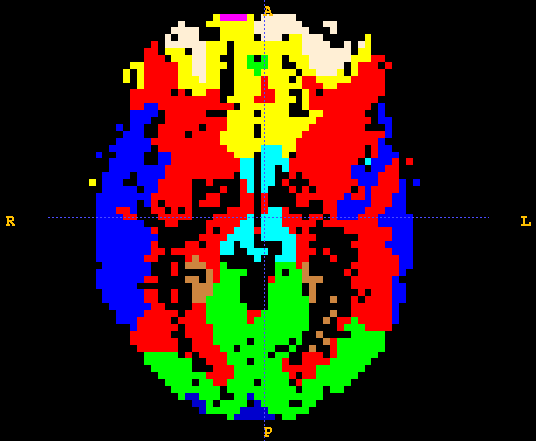
\includegraphics[width=0.3\textwidth]{figures/math/coherence/a}
  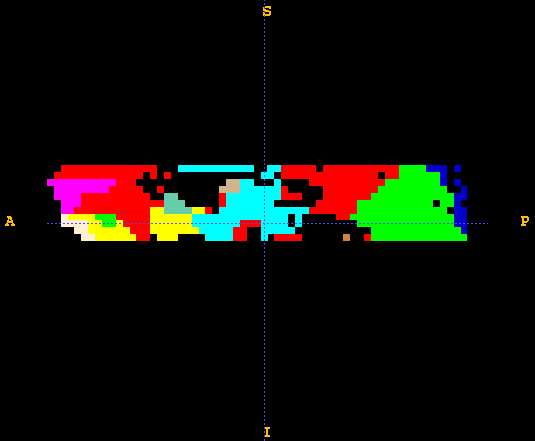
\includegraphics[width=0.3\textwidth]{figures/math/coherence/s}
  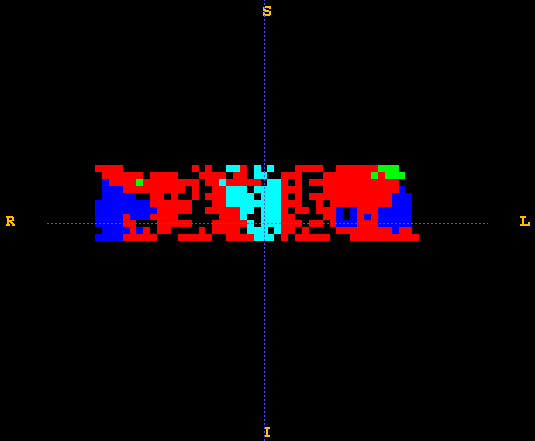
\includegraphics[width=0.3\textwidth]{figures/math/coherence/c}
  \caption{Segmentation map of a rs-fMRI volume. The spectral coherence between
    0.01 to 0.1 Hz is used for similarity between pairs of voxels. A spectral
    clustering method~\cite{von2007tutorial} is used for dimension reduction
    followed by a K-Means clustering. We choose 12 clusters and 10 slices on $z$
    direction to save computation time. }
  \label{fig:coherence}
\end{figure}

\begin{figure}[ptb]
  \centering
  \includegraphics[width=0.9\textwidth]{figures/c2/brain_graph}
  \caption{Using a graph to represent functional networks. A series of ROIs are chosen
    based on what questions  asked. Tthe signal at each ROI is computed by
    averaging the BOLD signals of all voxels within the sphere. The edge
    of the graph is estimated using the similarity of the signals between the
    ROIs. }
  \label{fig:brain_graph}
\end{figure}

\begin{figure}[ptb]
  \centering
  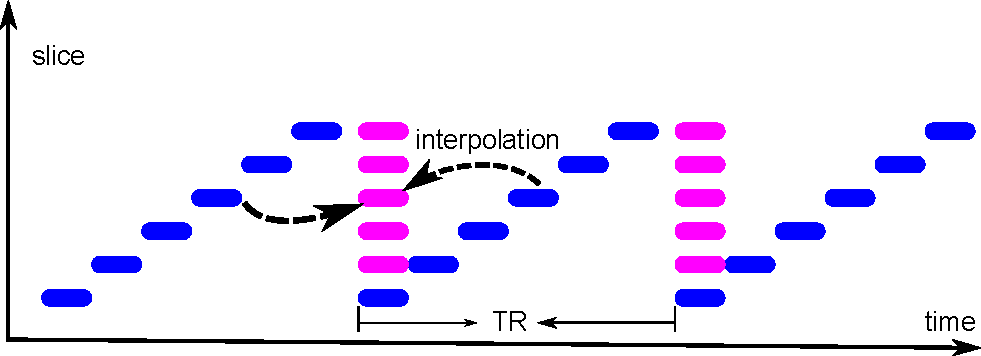
\includegraphics[width=0.9\textwidth]{figures/c2/slicetiming}
  \caption{Slice timing correction. The data at temporally adjacent slices are
    resampled and interpolated to obtain a data point at the same time with the
    reference slices.}
  \label{fig:slicetiming}
\end{figure}

\begin{figure}[ptb]
  \centering
  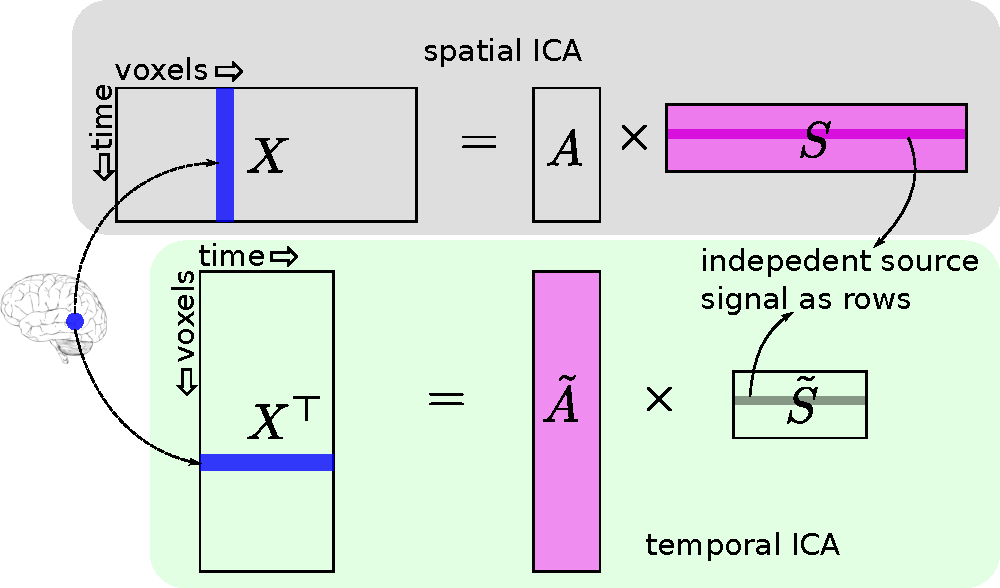
\includegraphics[width=0.8\textwidth]{figures/c2/ica}
  \caption{Spatial ICA versus temporal ICA for BOLD series of length $T$ at $N$
    voxels.  In spatial ICA, all the voxel intensity at a single time point is
    assumed to be a mixed signal of $P$ independent signals, and there are $T$ such
    mixed signals. The decomposition is in the form of $X = A\cdot S$, where A
    is the weight coefficient and each row of $S$ is the independent source
    signal.  We are interested in the $S$ since each row is regarded as a
    functional component. In temporal ICA, the BOLD time series of each voxel is
    the mixed signals, and there are $N$ such mixed signals. The decomposition
    is $\tilde X = \tilde A \cdot \tilde S$, with $\tilde A$ the weights, and
    rows in $\tilde S$ the independent signal. Here we are interested in the
    columns of $\tilde A$ as they are regarded as representations of the
    functional networks.  }
  \label{fig:c2ica}
\end{figure}

%%% Local Variables: 
%%% mode: latex
%%% TeX-master: "MyThesis"
%%% End: 

\chapter{Chapter 3 Title}\label{chap3}
%\fixchapterheading % Use this if section follows chapter immediately
Text

\section{Section Title}  % level 2
Text

\subsection{Subsection Title} %level 3
Text
\chapter{Chapter 4 Title}\label{chap4}
%\fixchapterheading % Use this if section follows chapter immediately
Text

\section{Section Title}  % level 2
Text

\subsection{Subsection Title} %level 3
Text
\numberofappendices=2   % Set 0 for none, else number of appendices.
\appendix       				% Chapters and sections are now appendix style
\chapter{Appendix Mean Field as Variation Inference}\label{appA}
%\fixchapterheading % Use this if section follows chapter immediately
Text

\section{Section Title}  % level 2
Text

\subsection{Subsection Title} %level 3
Text 

\chapter{Appendix B Title}\label{appB}
%\fixchapterheading % Use this if section follows chapter immediately
Text

\section{Section Title}  % level 2
Text

\subsection{Subsection Title} %level 3
Text 
%
% The choice of bibliography style is a major decision, jointly made
% by you, your thesis advisor and the thesis editor. Common choices are
% "siam", "acm", "amsplain", "plain", "chicago".
%

%Uncomment and use desired bibliography style
%\bibliographystyle{IEEEtran}
%\bibliography{MyThesisRefs}
\end{document}
